% Options for packages loaded elsewhere
\PassOptionsToPackage{unicode}{hyperref}
\PassOptionsToPackage{hyphens}{url}
%
\documentclass[
]{book}
\usepackage{amsmath,amssymb}
\usepackage{lmodern}
\usepackage{iftex}
\ifPDFTeX
  \usepackage[T1]{fontenc}
  \usepackage[utf8]{inputenc}
  \usepackage{textcomp} % provide euro and other symbols
\else % if luatex or xetex
  \usepackage{unicode-math}
  \defaultfontfeatures{Scale=MatchLowercase}
  \defaultfontfeatures[\rmfamily]{Ligatures=TeX,Scale=1}
\fi
% Use upquote if available, for straight quotes in verbatim environments
\IfFileExists{upquote.sty}{\usepackage{upquote}}{}
\IfFileExists{microtype.sty}{% use microtype if available
  \usepackage[]{microtype}
  \UseMicrotypeSet[protrusion]{basicmath} % disable protrusion for tt fonts
}{}
\makeatletter
\@ifundefined{KOMAClassName}{% if non-KOMA class
  \IfFileExists{parskip.sty}{%
    \usepackage{parskip}
  }{% else
    \setlength{\parindent}{0pt}
    \setlength{\parskip}{6pt plus 2pt minus 1pt}}
}{% if KOMA class
  \KOMAoptions{parskip=half}}
\makeatother
\usepackage{xcolor}
\usepackage{color}
\usepackage{fancyvrb}
\newcommand{\VerbBar}{|}
\newcommand{\VERB}{\Verb[commandchars=\\\{\}]}
\DefineVerbatimEnvironment{Highlighting}{Verbatim}{commandchars=\\\{\}}
% Add ',fontsize=\small' for more characters per line
\usepackage{framed}
\definecolor{shadecolor}{RGB}{248,248,248}
\newenvironment{Shaded}{\begin{snugshade}}{\end{snugshade}}
\newcommand{\AlertTok}[1]{\textcolor[rgb]{0.94,0.16,0.16}{#1}}
\newcommand{\AnnotationTok}[1]{\textcolor[rgb]{0.56,0.35,0.01}{\textbf{\textit{#1}}}}
\newcommand{\AttributeTok}[1]{\textcolor[rgb]{0.77,0.63,0.00}{#1}}
\newcommand{\BaseNTok}[1]{\textcolor[rgb]{0.00,0.00,0.81}{#1}}
\newcommand{\BuiltInTok}[1]{#1}
\newcommand{\CharTok}[1]{\textcolor[rgb]{0.31,0.60,0.02}{#1}}
\newcommand{\CommentTok}[1]{\textcolor[rgb]{0.56,0.35,0.01}{\textit{#1}}}
\newcommand{\CommentVarTok}[1]{\textcolor[rgb]{0.56,0.35,0.01}{\textbf{\textit{#1}}}}
\newcommand{\ConstantTok}[1]{\textcolor[rgb]{0.00,0.00,0.00}{#1}}
\newcommand{\ControlFlowTok}[1]{\textcolor[rgb]{0.13,0.29,0.53}{\textbf{#1}}}
\newcommand{\DataTypeTok}[1]{\textcolor[rgb]{0.13,0.29,0.53}{#1}}
\newcommand{\DecValTok}[1]{\textcolor[rgb]{0.00,0.00,0.81}{#1}}
\newcommand{\DocumentationTok}[1]{\textcolor[rgb]{0.56,0.35,0.01}{\textbf{\textit{#1}}}}
\newcommand{\ErrorTok}[1]{\textcolor[rgb]{0.64,0.00,0.00}{\textbf{#1}}}
\newcommand{\ExtensionTok}[1]{#1}
\newcommand{\FloatTok}[1]{\textcolor[rgb]{0.00,0.00,0.81}{#1}}
\newcommand{\FunctionTok}[1]{\textcolor[rgb]{0.00,0.00,0.00}{#1}}
\newcommand{\ImportTok}[1]{#1}
\newcommand{\InformationTok}[1]{\textcolor[rgb]{0.56,0.35,0.01}{\textbf{\textit{#1}}}}
\newcommand{\KeywordTok}[1]{\textcolor[rgb]{0.13,0.29,0.53}{\textbf{#1}}}
\newcommand{\NormalTok}[1]{#1}
\newcommand{\OperatorTok}[1]{\textcolor[rgb]{0.81,0.36,0.00}{\textbf{#1}}}
\newcommand{\OtherTok}[1]{\textcolor[rgb]{0.56,0.35,0.01}{#1}}
\newcommand{\PreprocessorTok}[1]{\textcolor[rgb]{0.56,0.35,0.01}{\textit{#1}}}
\newcommand{\RegionMarkerTok}[1]{#1}
\newcommand{\SpecialCharTok}[1]{\textcolor[rgb]{0.00,0.00,0.00}{#1}}
\newcommand{\SpecialStringTok}[1]{\textcolor[rgb]{0.31,0.60,0.02}{#1}}
\newcommand{\StringTok}[1]{\textcolor[rgb]{0.31,0.60,0.02}{#1}}
\newcommand{\VariableTok}[1]{\textcolor[rgb]{0.00,0.00,0.00}{#1}}
\newcommand{\VerbatimStringTok}[1]{\textcolor[rgb]{0.31,0.60,0.02}{#1}}
\newcommand{\WarningTok}[1]{\textcolor[rgb]{0.56,0.35,0.01}{\textbf{\textit{#1}}}}
\usepackage{longtable,booktabs,array}
\usepackage{calc} % for calculating minipage widths
% Correct order of tables after \paragraph or \subparagraph
\usepackage{etoolbox}
\makeatletter
\patchcmd\longtable{\par}{\if@noskipsec\mbox{}\fi\par}{}{}
\makeatother
% Allow footnotes in longtable head/foot
\IfFileExists{footnotehyper.sty}{\usepackage{footnotehyper}}{\usepackage{footnote}}
\makesavenoteenv{longtable}
\usepackage{graphicx}
\makeatletter
\def\maxwidth{\ifdim\Gin@nat@width>\linewidth\linewidth\else\Gin@nat@width\fi}
\def\maxheight{\ifdim\Gin@nat@height>\textheight\textheight\else\Gin@nat@height\fi}
\makeatother
% Scale images if necessary, so that they will not overflow the page
% margins by default, and it is still possible to overwrite the defaults
% using explicit options in \includegraphics[width, height, ...]{}
\setkeys{Gin}{width=\maxwidth,height=\maxheight,keepaspectratio}
% Set default figure placement to htbp
\makeatletter
\def\fps@figure{htbp}
\makeatother
\setlength{\emergencystretch}{3em} % prevent overfull lines
\providecommand{\tightlist}{%
  \setlength{\itemsep}{0pt}\setlength{\parskip}{0pt}}
\setcounter{secnumdepth}{5}
\usepackage{booktabs}
\usepackage{amsthm}
\makeatletter
\def\thm@space@setup{%
  \thm@preskip=8pt plus 2pt minus 4pt
  \thm@postskip=\thm@preskip
}
\makeatother
\ifLuaTeX
  \usepackage{selnolig}  % disable illegal ligatures
\fi
\usepackage[]{natbib}
\bibliographystyle{apalike}
\IfFileExists{bookmark.sty}{\usepackage{bookmark}}{\usepackage{hyperref}}
\IfFileExists{xurl.sty}{\usepackage{xurl}}{} % add URL line breaks if available
\urlstyle{same} % disable monospaced font for URLs
\hypersetup{
  pdftitle={Statistical Rethinking for Soil, Water, and Fish},
  pdfauthor={Josh Erickson},
  hidelinks,
  pdfcreator={LaTeX via pandoc}}

\title{Statistical Rethinking for Soil, Water, and Fish}
\author{Josh Erickson}
\date{2023-11-23}

\begin{document}
\maketitle

{
\setcounter{tocdepth}{1}
\tableofcontents
}
\hypertarget{the-golem-of-prague}{%
\chapter{The Golem of Prague}\label{the-golem-of-prague}}

Right now I'm just trying to work through what seems to be 4 years of reading statistical rethinking and learning statistics. Bare bones right now but hoping to make this more of a thing moving forward. Going to try and keep the context within a natural resource framework (fisheries, hydrology, soils).

I won't go into Chapter 1 because it's mostly for you to read on your own. Great content and outline for the rest of the book but not much to put on here.

\hypertarget{small-worlds-and-large-worlds}{%
\chapter{Small Worlds and Large Worlds}\label{small-worlds-and-large-worlds}}

\hypertarget{small-worlds-and-large-worlds-1}{%
\section{Small Worlds and Large Worlds}\label{small-worlds-and-large-worlds-1}}

A great distinction between the small and large world is the \emph{small world} is the model itself and the \emph{large world} is the world we hope to deploy in. This is the challenge of statistical modeling and is elevated by forgetting this distinction.

In the small world there are no surprises and it is important to verify the logic, making sure that it performs as expected under favorable assumptions.

The large world has events that were not expected or imagined in the small world, e.g.~coupling of events, a priori understanding is misleading, etc. This is essentially the modeling adage `all models are wrong, but some are useful'. Just because the model in the small world makes logical sense doesn't mean that it will be consistent in the large world. As Richard says, `But it is certainly a warm comfort.'

This chapter is where you'll start building Bayesian models. Bayesian models learn from prior information and this is super helpful in the small world. If this assumptions are close to reality, then they are also great in the large world.

\hypertarget{garden-of-forking-paths}{%
\subsection{Garden of forking paths}\label{garden-of-forking-paths}}

This is the humble beginnings of Bayesian inference: counting and comparing possibilities. Richard compares this to Jorge Luis Borges' short story ``The Garden of Forking Paths.'' In short, life is full of paths and exploring all of them will help make good inference. As we learn. We prune. This inference might not give a correct answer in the large world but it can guarantee the best possible answer in small world, given the information fed to it.

\hypertarget{counting-possibilities}{%
\subsubsection{Counting possibilities}\label{counting-possibilities}}

Here we'll take a play on the marble scenario but use fish in a bucket. Let's say you have a stream with either Bull Trout (\emph{salvelinus confluentus}) or Rainbow Trout (Oncorhynchus Mykiss) and let's say there are 4 samples from that stream. There are five different possibilities in these samples: some with all and some mixed,

\begin{verbatim}
## # A tibble: 4 x 5
##      p1    p2    p3    p4    p5
##   <dbl> <int> <int> <int> <dbl>
## 1     0     1     1     1     1
## 2     0     0     1     1     1
## 3     0     0     0     1     1
## 4     0     0     0     0     1
\end{verbatim}

\begin{figure}
\centering
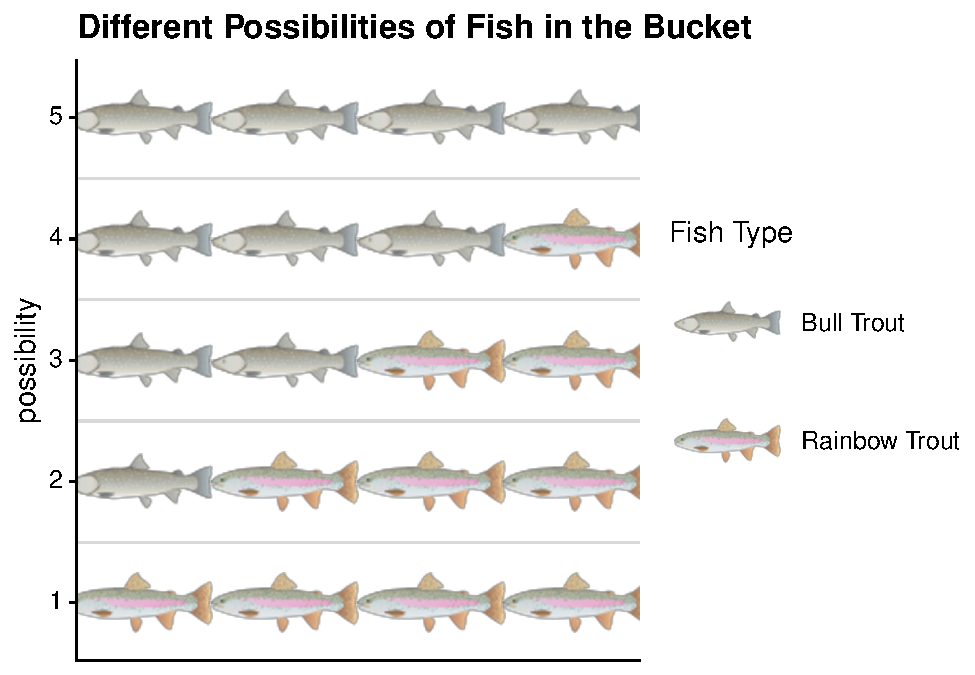
\includegraphics{bookdown-demo_files/figure-latex/figure-1-1.pdf}
\caption{\label{fig:figure-1}Possibilities in the bucket.}
\end{figure}

We want to figure out what conjecture is most plausible, given the evidence about the samples. Let's say that in the first 3 samples (with replacement) you get: Bull Trout, Rainbow Trout, Bull Trout (BT, RB, BT). Then what is the most plausible configuration in the bucket? Let's consider one example; \texttt{p2} (possibility \#2) from Figure \ref{fig:figure-1} (BT, RB, RB, RB). This is where the forking paths comes in handy because we can count the ways that this possibility can happen (Figure \ref{fig:figure-2}), i.e.~possibility meaning there is 3 RB and 1 BT in the bucket.

\begin{figure}
\centering
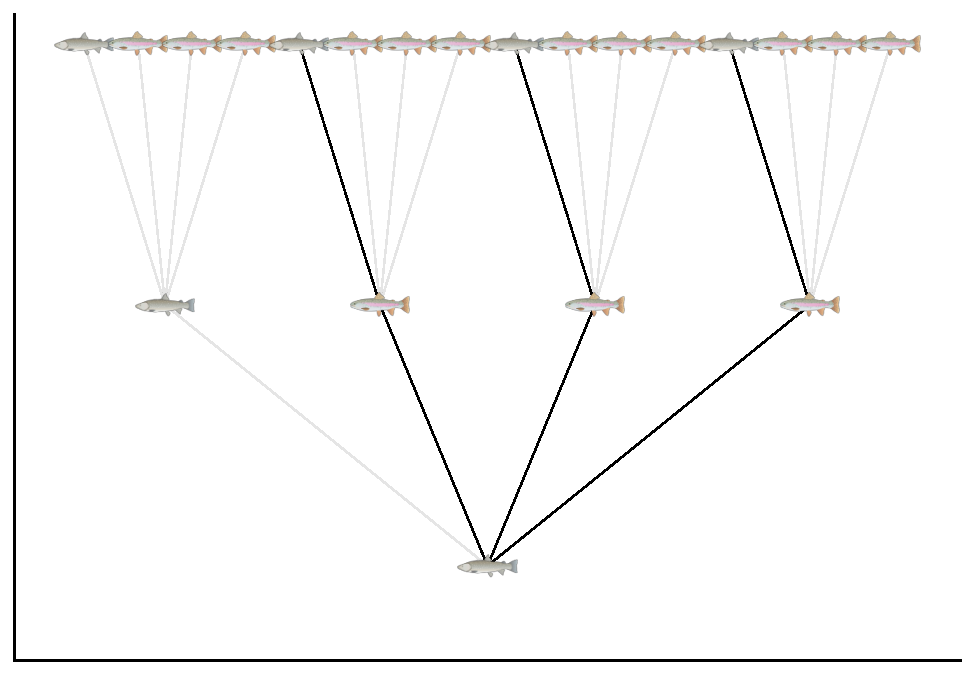
\includegraphics{bookdown-demo_files/figure-latex/figure-2-1.pdf}
\caption{\label{fig:figure-2}Paths taken in the bucket of forking fish.}
\end{figure}

In Figure \ref{fig:figure-2} above, we can see that there is 1 way of getting a bull trout in the first draw, 3 ways in the second and 1 again in the third. We can now do this for all the possibilities. Figure \ref{fig:figure-2} shows that there are 3 \emph{paths} or \emph{ways} for the bag to contain (BT, RB, RB, RB). Now this is great but we need to test all of the ways right? For example, let's say that we wanted to see if the bucket had all RB!? Right, that doesn't make sense. We pulled BT twice so this definitely isn't possible. Same goes for all BT. Since these paths don't exist based on our reality, we know that the way to produce them is 0. Now that we know the ways to produce (BT, RB, RB, RB) and the 0's, let's look at the others in Table \ref{tab:table-1} below.

\begin{table}

\caption{\label{tab:table-1}Conjectures and Ways to Produce Fish in a Bucket}
\centering
\begin{tabular}[t]{l|l|l|l|r|r|r|r}
\hline
p\_1 & p\_2 & p\_3 & p\_4 & draw 1: Bull Trout & draw 2: Rainbow Trout & draw 3: Bull Trout & ways to produce\\
\hline
BT & BT & BT & BT & 4 & 0 & 4 & 0\\
\hline
RB & BT & BT & BT & 3 & 1 & 3 & 9\\
\hline
RB & RB & BT & BT & 2 & 2 & 2 & 8\\
\hline
RB & RB & RB & BT & 1 & 3 & 1 & 3\\
\hline
RB & RB & RB & RB & 0 & 4 & 0 & 0\\
\hline
\end{tabular}
\end{table}

We can see based on our sample that (RB, BT, BT, BT) has 9 ways and (RB, RB, BT, BT) has 8 ways. These 5 different conjectures give us different \emph{paths} through the garden of forking data and tell us how we could produce (BT, RB, BT). As you can see in Table \ref{tab:table-1}, we just multiply the intermediary steps instead of counting but you'll see later that this is really handy when the conjectures grow.

\hypertarget{combining-other-information}{%
\subsubsection{Combining other information}\label{combining-other-information}}

What if we had information about the relative plausibility of each conjecture? Many ways we might have this but the important point is that it can help us to update these conjectures. In our case there's an easy solution: just multiply the counts.

Let's consider our initial data and call them \emph{priors}. Now let's say we draw another fish out of the bucket and it's a Bull Trout (BT). We could just start all over again and count the paths, etc or we could just multiply by the new observation and ways to produce it given the conjecture. It turns out these methods are mathematically identical (independent assumption). So to do this, we'll just take the \emph{prior} counts based on (BT, RB, BT) \textless=\textgreater{} (0, 3, 8, 9, 0) and multiply by the new ways (0, 1, 2, 3, 4) (Table \ref{tab:table-2}).

\begin{table}

\caption{\label{tab:table-2}Updating priors with new data.}
\centering
\begin{tabular}[t]{l|l|l|l|r|r|r}
\hline
p\_1 & p\_2 & p\_3 & p\_4 & Ways to Produce: Bull Trout & Prior counts & New count\\
\hline
BT & BT & BT & BT & 4 & 0 & 0\\
\hline
RB & BT & BT & BT & 3 & 9 & 27\\
\hline
RB & RB & BT & BT & 2 & 8 & 16\\
\hline
RB & RB & RB & BT & 1 & 3 & 3\\
\hline
RB & RB & RB & RB & 0 & 0 & 0\\
\hline
\end{tabular}
\end{table}

This is great because as new data arrives we can just update!

\hypertarget{from-counts-to-probability}{%
\subsubsection{From counts to probability}\label{from-counts-to-probability}}

This

\hypertarget{building-a-model}{%
\subsection{Building a Model}\label{building-a-model}}

The globe problem always reminded me of a similar hydrology problem with predicting headwater streams. We can look at the streams across the landscape similar to how we look at a tossing globe. First we need to sample a \emph{theoretical} stream network across a landscape and just like the globe if we get an observation on a stream or not we should be able to generate a posterior distribution. So let's bring in some data. We'll look at the NHDPLus High Resolution raster in Northwest Montana and sample from this raster to get an idea for a proportion of land to water.

\begin{Shaded}
\begin{Highlighting}[]
\FunctionTok{library}\NormalTok{(terra)}

\NormalTok{nhd }\OtherTok{\textless{}{-}} \FunctionTok{rast}\NormalTok{(}\StringTok{\textquotesingle{}Z:/GIT/stat\_rethinking/stat\_rethinking\_2023/nhdStrOrdRast.tif\textquotesingle{}}\NormalTok{)}
\NormalTok{sutton }\OtherTok{\textless{}{-}} \FunctionTok{vect}\NormalTok{(}\StringTok{\textquotesingle{}Z:/GIT/stat\_rethinking/stat\_rethinking\_2023/sutton.shp\textquotesingle{}}\NormalTok{) }\SpecialCharTok{\%\textgreater{}\%} \FunctionTok{project}\NormalTok{(}\FunctionTok{crs}\NormalTok{(nhd))}
\NormalTok{nhd\_sutton }\OtherTok{\textless{}{-}} \FunctionTok{crop}\NormalTok{(nhd, sutton, }\AttributeTok{mask =}\NormalTok{ T)}

\FunctionTok{plot}\NormalTok{(nhd\_sutton, }\AttributeTok{col =} \StringTok{\textquotesingle{}blue\textquotesingle{}}\NormalTok{)}
\FunctionTok{plot}\NormalTok{(sutton, }\AttributeTok{add =} \ConstantTok{TRUE}\NormalTok{, }\AttributeTok{fill =} \ConstantTok{NA}\NormalTok{)}
\end{Highlighting}
\end{Shaded}

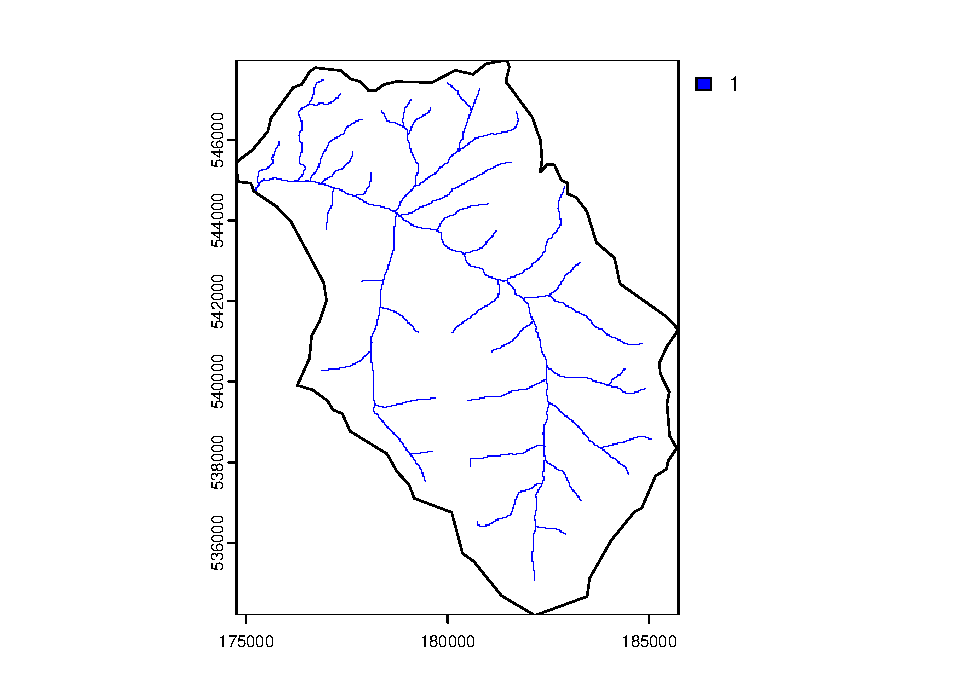
\includegraphics{bookdown-demo_files/figure-latex/unnamed-chunk-1-1.pdf}

\begin{Shaded}
\begin{Highlighting}[]
\FunctionTok{set.seed}\NormalTok{(}\DecValTok{1234}\NormalTok{)}

\NormalTok{sample9 }\OtherTok{\textless{}{-}}\NormalTok{ terra}\SpecialCharTok{::}\FunctionTok{spatSample}\NormalTok{(nhd\_sutton, }\AttributeTok{size =} \DecValTok{9}\NormalTok{, }\AttributeTok{method =} \StringTok{"random"}\NormalTok{, }\AttributeTok{replace =} \ConstantTok{TRUE}\NormalTok{)}

\DocumentationTok{\#\# just adding a S and L}
\NormalTok{sample9}\SpecialCharTok{$}\NormalTok{observations }\OtherTok{\textless{}{-}} \FunctionTok{ifelse}\NormalTok{(}\FunctionTok{is.na}\NormalTok{(sample9}\SpecialCharTok{$}\NormalTok{nhdStrOrdRast), }\StringTok{\textquotesingle{}Land\textquotesingle{}}\NormalTok{, }\StringTok{\textquotesingle{}Stream\textquotesingle{}}\NormalTok{)}
\end{Highlighting}
\end{Shaded}

In this example we'll randomly sample this stream raster to get a sample of S (stream) or L (land). So from the vector \texttt{sample9} we get Land, Land, Land, Land, Land, Land, Stream, Land, Land.

As you can see it's pretty rare to get a stream with all that land!

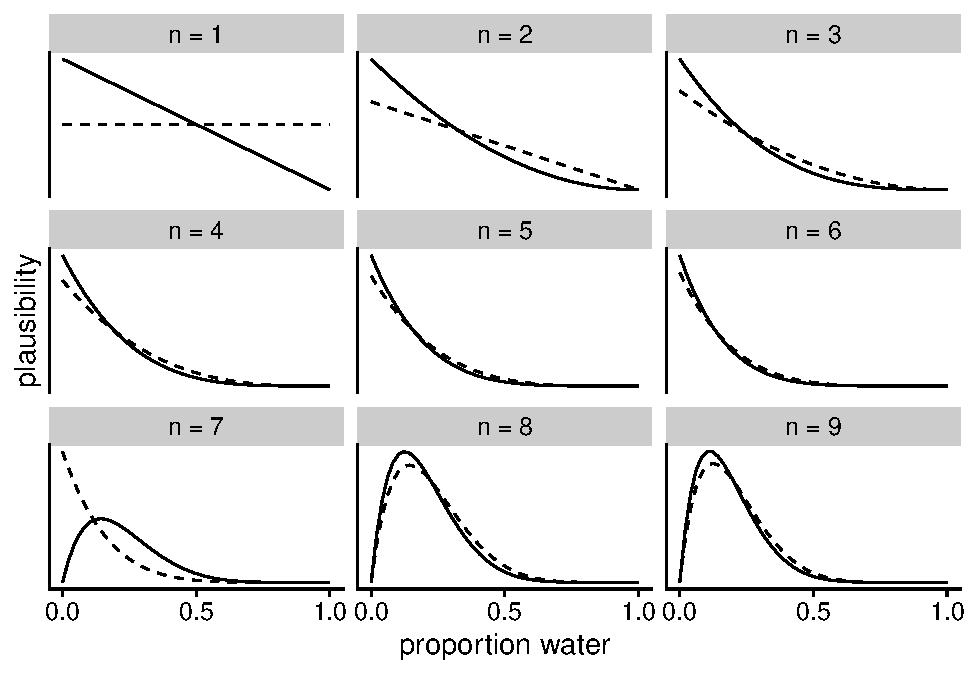
\includegraphics{bookdown-demo_files/figure-latex/unnamed-chunk-2-1.pdf}

So we can see from the graph above that we are taking a 50\% probability of getting `S' or `L' (even though we know that's not true\ldots) and then updating based on our sample of Land and Stream. So every time \texttt{Land} is observed, the peak of the plausibility curve moves to the left in the graph. Now that we've seen the model we can just use the \texttt{dbinom()} to find the probability.

\begin{Shaded}
\begin{Highlighting}[]
\FunctionTok{dbinom}\NormalTok{(}\DecValTok{1}\NormalTok{, }\AttributeTok{size =} \DecValTok{9}\NormalTok{, }\AttributeTok{prob =}\NormalTok{ .}\DecValTok{5}\NormalTok{)}
\end{Highlighting}
\end{Shaded}

\begin{verbatim}
## [1] 0.01757813
\end{verbatim}

This is the relative number of ways to get 1 stream, holding \(p\) at 0.5 and \(N = W+L\) at 9. We can now summarize our model.\\

\[
W \sim \text{Binomial}(N,p)
\]
And the unobserved parameter \(p\) gets:

\[
p \sim \text{Uniform}(0,1)
\]
This is not the best prior since we know this area has way more land to stream.

\hypertarget{making-the-model-go}{%
\subsection{Making the model go}\label{making-the-model-go}}

A Bayesian model can update all of the prior distributions to their purely logical consequences: the Posteriro Distribution. This distribution contains the relative plausibility of different parameter values, conditional on the data and model, e.g.~probability of the parameters, conditional on the data \(Pr(p|W,S)\). This means the probability of each possible value of \(p\), conditional on the specific \(S\) and \(L\) that we observed.

Bayes' theorem:

\[
Pr(S, L, p) = Pr(S, L|p)Pr(p)
\]

Now just reverse the \(p\) on the \(rhs\).

\[
Pr(S, L, p) = Pr(p|S, L)Pr(S,L)
\]

Not that these are equal to the same thing we can just equal them to each other.

\[
Pr(p|S,L)=\frac{Pr(S, L|p)Pr(p)}{Pr(S,L)}
\]
\[
\text{Posterior}=\frac{\text{Probability of the data} \times \text{Prior}}{\text{Average probability of the data}}
\]

\hypertarget{sampling-the-imaginary}{%
\chapter{Sampling the Imaginary}\label{sampling-the-imaginary}}

We describe our methods in this chapter.

Math can be added in body using usual syntax like this

\hypertarget{math-example}{%
\section{math example}\label{math-example}}

\(p\) is unknown but expected to be around 1/3. Standard error will be approximated

\[
SE = \sqrt(\frac{p(1-p)}{n}) \approx \sqrt{\frac{1/3 (1 - 1/3)} {300}} = 0.027
\]

You can also use math in footnotes like this\footnote{where we mention \(p = \frac{a}{b}\)}.

We will approximate standard error to 0.027\footnote{\(p\) is unknown but expected to be around 1/3. Standard error will be approximated

  \[
  SE = \sqrt(\frac{p(1-p)}{n}) \approx \sqrt{\frac{1/3 (1 - 1/3)} {300}} = 0.027
  \]}

  \bibliography{book.bib,packages.bib}

\end{document}
